\documentclass[]{iosart2c}
% \usepackage[T1]{fontenc}
\usepackage[utf8]{inputenc}
\usepackage[a4paper,width=160mm,top=20mm,bottom=15mm,right=0mm]{geometry}
\usepackage{times,mathtools, amssymb, amsfonts, amsmath, fancyhdr, graphics, dcolumn, natbib, graphicx}
\usepackage{algorithm}
\usepackage[noend]{algpseudocode}
\usepackage[switch]{lineno}
\usepackage[none]{hyphenat}
\usepackage{microtype}
% \usepackage[style=apa,backend=biber,bibencoding=latin1]{biblatex}
% \addbibresource{output.bib}

\renewcommand{\algorithmicrequire}{Input:}
\renewcommand{\algorithmicensure}{Output:}

\linenumbers
\renewcommand{\baselinestretch}{1.1}
\setlength{\parskip}{.5em}

\pagestyle{fancy}
\renewcommand{\headrulewidth}{0.4pt}
\renewcommand{\footrulewidth}{0.4pt}
\fancyhead{}
\fancyhead[RO,LE]{Thesis Title}
\fancyfoot{}
\fancyfoot[LE,RO]{\thepage}
\fancyfoot[LO,CE]{Chapter \thechapter}
\fancyfoot[CO,RE]{Author Name}

\def\QEDmark{\ensuremath{\square}}
\def\proof{

  \paragraph{\textbf{Proof}.}}
\def\endproof{\hfill\QEDmark}

\graphicspath{ {./images/} }

\begin{document}

  \begin{frontmatter}

    \title{A distance-based approach for merging\\
    probabilistic knowledge bases}

    \runningtitle{A distance-based approach for merging probabilistic knowledge bases}

    \author[A,C]{\fnms{Van Tham} \snm{Nguyen}},
    \author[B,D]{\fnms{Ngoc Thanh} \snm{Nguyen}}
    and
    \author[A]{\fnms{Trong Hieu} \snm{Tran}%
    \thanks{Corresponding author. Trong Hieu Tran, Faculty of Information Technology, Nguyen Tat Thanh University,
      Ho Chi Minh city, Vietnam. hieutt@vnu.edu.vn}}

    \runningauthor{V.T. Nguyen et al.}

    \address[A]{University of Engineering and Technology, Vietnam National University, Hanoi, Vietnam}
    \address[B]{Faculty of Computer Science and Management, Wroclaw University of Science and Technology, Poland}
    \address[C]{Faculty of Information Technology, Namdinh University of Technology Education, Vietnam}
    \address[D]{Faculty of Information Technology, Nguyen Tat Thanh University, Ho Chi Minh city, Vietnam}

    \begin{abstract}
      In the stages of development of probabilistic expert systems, knowledge merging is a major concern. To deal with
      knowledge merging problems, several approaches have been put forward. However, in the proposed models, each
      original probabilistic knowledge base (PKB) is represented by a set of probabilistic functions fulfilling such
      knowledge base. The drawbacks of the solutions are that the output of model is also a set of probabilistic
      functions satisfying the resulting PKB and there is no algorithm for implementing the merging process of PKBs in
      which each of them consists of probabilistic constraints. In this paper, distance-based approach is utilized to
      propose a new method of merging PKBs to ensure that both the input and output of methods are represented by sets
      of probabilistic constraints. To this aim, the relationship between the probability rules and the probabilistic
      constraints, and the several transformation methods for the representation of the original PKB are presented, a
      set of merging operators (MOs) is proposed, and several desirable logical properties are investigated and
      discussed. Several algorithms for merging PKBs are presented and the computational complexities of these
      algorithms are also analyzed and evaluated

    \end{abstract}

    \begin{keyword}
      Probabilistic knowledge base, knowledge merging, merging operator, algorithm
    \end{keyword}

  \end{frontmatter}

  \thispagestyle{empty}
  \pagestyle{empty}


  \section{Introduction}
  Improving appropriate methods to build and maintain the action of knowledge-based systems is very necessary. In
  security systems, advanced methods of symbolic knowledge representation are used to integrate different, distributed
  source of information and in this way to make a system be flexible and more effective \cite{1}. It is necessary to
  transform information stored in knowledge bases when two computer systems need to be integrated or when they exchange
  content of their knowledge bases \cite{2}. In order to ensure that systems could interact with each other, the
  knowledge bases originating from these systems have to be consistent. Knowledge merging could be understood as a
  process of creating a consistent knowledge from a set of knowledge bases deriving from different systems \cite{3}.
  Knowledge merging is an important problem and its applications are many and diverse. The process of merging could
  require that knowledge bases should change to ensure the consistency of the merged knowledge base. Therefore, it is
  a difficult problem and considering these changes is very essential. Knowledge merging could be observed in two
  respects: Merging knowledge bases which are not similar and merging a set of different representations for same
  knowledge base but different in representing degree \cite{3}. Therefore, the first task in the knowledge merging
  process is to solve the inconsistency in knowledge bases. A data filling approach for incomplete set in which missing
  data is filled in terms of the probability of objects appearing in the mapping sets of parameters could find in
  \cite{4}. A class of basic inconsistency measures for probabilistic framework has been introduced in \cite{5}
  \cite{6}. In a probabilistic environment, some strategies have been developed to deal with the inconsistency of a
  knowledge base. The method of modification of probabilities is one of the most common approaches. This method has
  been applied in \cite{7} \cite{8} \cite{9} \cite{10}.

  A general model of knowledge merging problem referring to its inconsistency in distribution aspect was introduced in
  \cite{3}. In this work, the author worked out and discussed the knowledge merging problem, postulates for knowledge
  merging and algorithms for this process. In a logic environment, some approaches were proposed to merge propositional
  knowledge \cite{11} \cite{12} \cite{13}. The main idea of those strategies is often to build a family of MOs:
  Model-based operators and Formula-based MOs \cite{11}, DA2 MOs \cite{12}, MOs (Quota, Gmin) \cite{13}. MOs in
  \cite{11}, \cite{12} are built in the propositional logic framework and they require all the knowledge bases have the
  same importance, priority, or easibility. Moreover, model-based operators cannot take into account inconsistent
  knowledge bases, but in some cases the information from these bases can be useful while the drawback of formula-based
  MOs is that the sources of information could be lost in the merging process.

  It can be necessary to merge knowledge bases with more structure than the one of propositional logic. In this case
  weighted approaches are the best way. This is usually represented using possibilistic logic. For possibilistic
  knowledge merging issue, there are many different methods [14–16] proposed to solve. Merging process of these
  methods includes two stages: the separation and the combination. In the first step, each knowledge base is divided
  into two sub-bases and then the combination step employs different operators to combine different classes of
  sub-bases. However, there is no possibilistic merging operator satisfying all the postulates for merging possibilistic
  knowledge bases \cite{16}. Another method proposed in \cite{17} state that keeping weighted information after merging
  is not always necessary. The models of this work are models of the formula representing the integrity constraints
  that are maximal with respect to the lexicographic ordering. However, the drawback of the solutions is that the work
  does not present a representation theorem for the generalized postulates.Moreover, the merging results are usually
  consistent when using the propositional MOs, while the merging results may be inconsistent if using the possibilistic
  MOs.

  Within the probabilistic framework, knowledge merging is understood as a process of building a joint probability
  distribution from an input set of low-dimensional distributions [18–20]. The main purpose of this work is to create
  a unifying framework for operations with probability distributions that would be used for description of iterative
  procedures for proposing solving methods. However, the convergence of those algorithms in \cite{18} \cite{19} \cite{20} have not been
  carefully considered. Another approach is to build MOs based on convex Bregman divergences. A family of probabilistic
  MOs was first introduced in \cite{21} and they were further studied in \cite{22} \cite{23}. These operators were discussed,
  evaluated, and compared to each other in detail in \cite{23}. However, the main limitation of approaches proposed
  in \cite{21} \cite{22} \cite{23} is that it only works with PKBs represented by probability functions.

  In the previous work \cite{24}, the representation of PKB by probability functions and divergence distance functions
  is taken into account. A deeply survey is first made on how to compute a set of probability functions satisfying PKB,
  then the way these functions could be employed to merge probabilistic knowledge bases by proposing two MOs based on
  divergence distance functions has also been shown. Satisfied probabilistic functions correspond to convex optimization
  problems or linear programs while all these operators correspond to convex optimization problems. However, the
  propositions and examples are given but there is no proofs nor algorithms to implement the merging process. Moreover,
  the output of the proposed model is only the probabilistic functions representing newly merged knowledge base being
  not represented in the same form as the original knowledge bases.

  This paper is extended from our conference paper \cite{24}. It introduces in more details how to calculate a set of
  probability functions satisfying a PKB, probability merging vector as well as the new probability of constraints in
  merged PKB. Comparing with the conference paper our contributions are based on the fact that propositions for
  calculating such values are proved by pointing that there always exists optimal solutions \cite{25} and the output of
  merged PKB is similar to original PKBs in representation. Besides, main algorithms using to merge PKBs have been put
  forward by obeying probability rules and condition property of MOs. In addition to pointing out that proposed
  operators fulfill several desirable properties, two new operators is investigated more and unproven remaining
  statements have also been made. Finally, a simple but explanatory example to illustrate, analyze and evaluate
  computational complexity of proposed algorithms is presented.

  The rest of this paper is organized as follows. The second section presents the related work on approaches for
  merging PKBs. Some basic notions about probability function, probabilistic constraint, probability rules, the
  representation of knowledge bases in a probabilistic framework, and a PKB profile for such bases are presented in
  the third section. The subsequent section gives distance-based probabilistic MOs. The way to determine probabilistic
  merging vector as well as the desirable logical properties for MOs are also drawn and discussed in this section.
  Algorithms for merging PKBs as well as the analysis and evaluation of these algorithms are presented in the next
  sections. The final section will conclude the main results that have been investigated and give some future works.


  \section{Related work}

  The problem of merging PKBs has been studied for a long time and gets a lot of attention in recent years. The idea of probabilistic merging has been introduced and discussed in detail by Vomlel \cite{18} . This work proposed a design and characterization of methods applicable to the merging process of knowledge bases represented by a set of probability distributions. Vomlel used the means of the Iterative Proportional Fitting Procedure (IPFP) to build a joint probability distribution from an input set of low-dimensional distributions. In the case of inconsistent input set, five iterative methods were proposed, namely: CC LCC, AA, GA, and GEM. In the case of consistent input set, iterative proportional fitting procedure have the best convergence rate of five iterative methods for inconsistent input set. However, several properties of methods were not proven and not achieved in this general case due to problems with probability distributions containing zeroes. Vomlel continued proposing another method that extends IPFP to deal with inconsistent constraints, named GEMA \cite{19}. It generalizes the concept of expectation maximization. The time performance of GEMA was extremely sensitive to both the initial knowledge bases and the constraints. As full joint distributions were directly manipulated by GEMA, the advantages of other probabilistic models such as the Bayesian networks (BNs) could be taken. In order to overcome these limitations, Zhang et al. \cite{20} proposed another algorithm called Smooth which addressed both consistent and inconsistent constraints. However, the convergence of Smooth was only proven empirically through experiments. Therefore, the key drawback of the approaches [18–20] is that PKBs must be represented by probability distributions.

  Adamcik \cite{23} associated the geometrical notion of projections by means of a Bregman divergence with the framework of pooling operators to solving the problem of probabilistic knowledge merging. A class of MOs based on minimization of a sum of convex Bregman divergences was introduced and proposed. The most common model of merging operator was defined by

  $\Delta (\mathcal{K}_1, ... ,\mathcal{K}_n) = \{ \arg \min_{v \in D^L} H(w^{(i)}||v) : w^{(i)} \in V^L_{K_i}\}$

  where L is a finite propositional language, $D^L$ is the set of all probability functions over, H is a Bregman divergence function and each PKB $\mathcal{K}_i$ for $1 \le i \le n$ over L is a set of constraints on probability functions over L such that the set of all probability functions satisfying the constraints in $K_i$ forms a nonempty closed convex subset $V^L_{K^i}$ of DL. The ˆ$\Delta D$ -merging operator was defined by using Squared Euclidean Distance and extending the LinOp-pooling operator, in the sense that it coincides with LinOp in the special case when each knowledge base admits only a single probability function. The linear Entropy Operator was defined by using Kullback-Leibler Divergence while the Linear Renyi Operator was employed Renyi Divergence. The linear Entropy Operator was similar to the Linear Euclidean Operator built by Osherson and Vardi in \cite{26} and contained reversed parameter compared to Social Entropy Operator proposed by Wilmers in \cite{21}. Adamcik also showed that MOs satisfied the natural principle of consistency. However, original PKBs and resulting knowledge base in this work were only represented by probabilistic functions and placed in the context of the propositional language. Moreover, more general applications as well as the rate of convergence of the algorithm need to be carefully investigated.

  The new approach proposed in this paper is compared with existing ones given in the literature. Like the merging methods given in [18, 21, 23, 26], this 2 new approach also employs distance functions to find a set of probability functions representing common PKB. However, the first difference is that some propositions introduced in [9, 10] are applied to find probabilistic functions satisfying original PKB that is represented by probabilistic constraints. The second difference is that probability rules proposed \cite{27} are employed to find new value of probabilistic constraints in common PKB.


  \section{Basic notions}

  A sample space, denoted by $\mathcal S$, is a set which includes all possible outcomes of a statistical experiment. A finite set of possible outcomes forms an event. A set of events denoted by $\hat{\varepsilon}$, $\hat{\varepsilon} = \{ E _1, ... , E_n \}$. Given $F,G \in \hat{\varepsilon}$ , the intersection $F$ and $G$, denoted by $F \cap G$, is an event which contains all elements that are common to $F$ and $G$; the negation of event $F$, denoted by $\neg F$, is abbreviated by $\neg F$ . A complete conjunction of $\hat{\varepsilon}$ denoted by $\Theta$,$\Theta = \tilde E1 \cap \tilde E2 \cap ... \cap \tilde E_n$ where $\tilde E_i = {E_i, \neg E_i}$. A set of all complete conjunctions of $\hat{\varepsilon}$, denoted by $\wedge (\hat{\varepsilon}),\wedge (\hat{\varepsilon}),= {\Theta_i, ... , \Theta_{2^n}  }$. A complete conjunction $\Theta \in \wedge (\hat{\varepsilon} )$ satisfies an event $F$, denoted by $\Theta \Delta \models F$, iff  $F$ appears in $\Theta$. Also, it said that $\Theta \Delta \models {E_i, ... , E_n}$ if $\Theta \Delta \models E_i, \forall 1 \le i \le n$. Let $f\mho (X) = {\Theta \in \Delta (\hat{\varepsilon} )|\Theta \Delta \models X}$, where $X$ is an event or a set of events. Let $m = |\Lambda(\hat{\varepsilon})| = 2n$ be the numbers of complete conjunctions of $\hat{\varepsilon}$ . Let $\mathbb{R}_{\geq0}$ be the set of non-negative real values including $+\infty$. Let $\mathbb{R}_{[0,1]}$ be the set of all real values from 0 to 1.


  \textbf{Definition 1}. Let $\mathcal{P} : \Lambda(\hat{\varepsilon}) \to \mathbb{R}_{[0,1]}$ such as,
  $\sum_{i=1}^m \mathcal{P} (\Theta i) = 1$, $\mathcal{P}$ is called a probability function.
  Let $\hat{\mathcal{P}} (\hat  \varepsilon )$ be a set of all probability functions $\mathcal{P}$ over set of events $\hat  \varepsilon$, defined by $\hat{\mathcal{P}}(\hat  \varepsilon) =  {\mathcal{P} (\Theta1), ... ,\mathcal{P} (\Theta_{2^n} )}$. Let $\vec{\vartheta} = (\vartheta_1, ... , \vartheta_m)^T$ be a column vector, where an auxiliary variable $\vartheta_i$ corresponding to a probability $\mathcal{P}(\Theta_i)$.


  \textbf{Proposition 1}. \textit{Let $F,G \in \hat{\varepsilon}$ Probability function $\mathcal{P}$ satisfies the following probability axioms}:

  (\textbf{P0}) $\mathcal{P}(F) = \sum_{\Theta  \in  \Lambda (\hat{\varepsilon}):\Theta  \models F}\mathcal{P}(\Theta)$

  (\textbf{P1}) $\mathcal{P} (FG) = \mathcal{P} (F) \mathcal{P} (G/F) = \mathcal{P} (G) \mathcal{P} (F/G)$ provided $\mathcal{P} (G) > 0,\mathcal{P} (F) > 0$

  (\textbf{P2}) $\mathcal{P}(G_k|F) = \frac{\mathcal{P}(G_k)\mathcal{P}(F|G_k)}{\sum_{i=1}^{n} \mathcal{P}(G_i)\mathcal{P}(F|G_i)} \forall k = 1, ..., n$

  (\textbf{P3}) $\mathcal{P}(F) = \sum_{i=1}^{n} {\mathcal{P}(G_i)\mathcal{P}(F|G_i)}$

  (\textbf{P4}) $\mathcal{P}(F) = 1 - \mathcal{P}(\overline F)$

  \textit{Any countable sequence of disjoint sets (synonymous with mutually exclusive events) $F_1, F_2, ... F_n$ satisfies}

  (\textbf{P5}) $\mathcal{P}(\cup_{i=1}^\infty F_i) = \sum_{i=1}^n \mathcal{P}(F_i)$

  \begin{proof}
    Axiom \textbf{P0} may be inferred easily from the Definition 1. Axiom \textbf{P1} is the result of Definition 2.10, axiom \textbf{P2} is the result of Theorem 2.14, axiom \textbf{P3} is the result of Theorem 2.13, axiom \textbf{P4} is the result of Theorem 2.9, axiom \textbf{P5} is the result of Corollary 2.2, which were proposed and proved in \cite{27}.
  \end{proof}


  \textbf{Definition 2}. Let $F,G \in \hat{\varepsilon}$ and $\rho \in \mathbb{R}_{[0,1]}$. A probabilistic constraint is an expression of the form $c[\rho]$,where $c = (F|G)$.

  Intuitively, a constraint $(F|G)[\rho]$ means that our knowledge in $F$ given that $G$  hold has probability value $\rho$. If $F$ does not depend on $G,G \equiv _\top, (F|_\top)[\rho]$, is abbreviated by $(F)[\rho]$.

  \textbf{Definition 3}. A PKB, denoted by $\mathcal{K} = \langle \kappa_1, ... \kappa kh \rangle$, is a finite set of probabilistic constraints, where $\kappa i = c_i[\rho_i]$ for all $i = 1, ... h$.

  Let $h = |\mathcal{K}|$ be the total number of constraints in $\mathcal{K}$. A probability function $\mathcal{P} \in \hat{\mathcal{P}} (\hat{\varepsilon})$ satisfies a probabilistic constraint $c[\rho]$, denoted by $\mathcal{P} \models c[\rho]$ iff $\mathcal{P}(FG) = \rho\mathcal{P}(G)$. A probability function $\mathcal{P}$ satisfies $\mathcal{K}$ denoted by $\mathcal{P} \models \mathcal{K}$ iff $\mathcal{P} \models \mathcal{K}\forall \mathcal{K} \in \mathcal{K}$. Let $\mho (\mathcal{K}) = {\mathcal{P} \in \hat{\mathcal{P}} (\hat{\varepsilon})|\mathcal{P} \models \mathcal{K}}$ be the set of all probability function values satisfying $\mathcal{K}$. The set of constraints of $\mathcal{K}_1 \cup \mathcal{K}_2$ corresponds to $\mho(\mathcal{K}_1 \cup \mathcal{K}_2) = \mho(\mathcal{K}_1) \cap \mho (\mathcal{K}_2)$.

  \textbf{Definition 4}. Let $\mathbb{K}$ be a set of PKBs. Inconsistency measure $\mathcal{J}M$ is a function $\mathcal{J}M: \mathbb{K} \to \mathbb {R}_{\geq 0}$ such that $\mathcal{J}M(\mathcal{K}) = 0$ if and only if $\mho (\mathcal{K}) \neq \emptyset, \mathcal{K} \in \mathbb{K}$.

  \textbf{Definition 5}. A PKB $\mathcal{K}$ is consistent, denoted by $\nvDash \perp$, iff $\mho (\mathcal{K}) \neq \theta$. Otherwise, $\mathcal{K}$ is inconsistent, denoted by $\mathcal{K} \models \perp$.

  \textbf{Definition 6}. A PKB profile, denoted by $\mathcal{B} = {\mathcal{K}_1, ...\mathcal{K}_n}$ is a finite set of PKBs satisfying the following conditions:

  \begin{enumerate}

    \item $\forall \mathcal{K}_i \in \mathcal{B} : \mathbb{K}_i \nvDash \perp$
    \item $\forall \mathcal{K}_i,\mathcal{K}_j (i \neq j) :$\\
    $+|\mathcal{K}_i| = |\mathcal{K}_j|$ \\
    $+\forall c_k[\rho k] \in \mathcal{K}_i; c'_{k'} [\rho k'] \in \mathcal{K}_j; k = k' : c_k = c'_{k'}$\\
    $\mathcal{K}_i$ is consistent to $\mathcal{K}_2$ iff they satisfy condition 2, denoted by $\mathcal{K}_1||\mathcal{K}_2$. Otherwise, $\mathcal{K}_1 \nparallel \mathcal{K}_2$.

  \end{enumerate}


  \section{Distance-based probabilistic MOs}

  \subsection{Desirable properties}

  In the rest later, several properties of our family of probabilistic MOs used to characterize MOs will be put forward. Let be a function $\Gamma: \mathcal{B} \to \mho(\mathcal{B})$ that maps a PKB profile onto a set of all probability function values satisfying $\mathcal{B}$. The following definition is similar to a set of logical properties which was stated in [3, 28].

  \textbf{Definition 7}. Let $\mathcal{B} = \{\mathcal{K}_1 , ... ,\mathcal{K}_n\}$ and, $\mathcal{C} = \{\mathcal{K}_1, ... ,\mathcal{K}_m\}$ be PKB profiles. Let $\mathcal{K}$ be a consistent PKBs. Function $\Gamma: \mathcal{B} \to \upsilon(\mathcal{B})$ is called a probabilistic merging operator iff the following properties hold:

  (\textbf{CP1}) \textit{Consistency Principle. If $\cap^n_{i=1}\mho(\mathcal{K}_i) \neq \emptyset$ then $\Gamma(\mathcal{B}) \subseteq \cap^n_{i=1}\mho(\mathcal{K}_i)$
    The property CP1 assures that if the input PKB profile is consistent then the result of merging will be a subset of the intersection of the set of all probability function values satisfying $\mathcal{K}_i$.}

  (\textbf{SCP}) \textit{Strong Consistency Principle. If $\cap^n_{i=1}\mho(\mathcal{K}_i) \neq \emptyset$ then $\Gamma(\mathcal{B}) = \cap^n_{i=1}\mho(\mathcal{K}_i)$}

  \textit{The property SCP assures that if the input PKB profile is consistent then the result of merging will be the intersection of the set of all probability function
  values satisfying $\mathcal{K}_i$.}

  (\textbf{IP}) \textit{Ignorance Principle. $\forall \mathcal{K} = \emptyset : \Gamma(\mathcal{B} \cup \mathcal{K}) = \Gamma(\mathcal{B})$}

  \textit{The property IP state that the result of merging process should not be affected when an empty PKB is added.}

  (\textbf{EP}) \textit{Equivalence Principle. If there exists a permutation $\mu on {1, ... , n}$ such that $\Omega(\mathcal{K}_i) = (\mathcal{K}_\mu(i))$ then $\Gamma(\mathcal{B}) =  \Gamma(\mathcal{C})$}

  \textit{The property EP implies that result of merging process should not be contingent on the occurrence order of PKBs.}

  (\textbf{CP2}) Collegiality Principle. If $\cap^m_{i=1|\mho(\mathcal{K}_i} \neq \emptyset$ and $\Gamma(\mathcal{B}) \subseteq \cap^m_{i=1}\mho(\mathcal{K'_i})$ then $\Gamma(\mathcal{B} \cup \mathcal{C}) + \Gamma(\mathcal{B})$.

  \textit{The property CP2 implies that the result of merging process should not be affected when a PKB profile which the intersection of the set of all probability function values satisfying $\mathcal{K}_i$ in it contains the merging result of other is added.
  }
  (\textbf{AP}) \textit{Agreement. If $(\mathcal{B}) \cap (\mathcal{C}) \neq \emptyset$ then $(\mathcal{B}) \cap (\mathcal{C}) = (\mathcal{B} \cup \mathcal{C})$.}

  \textit{This property states that the intersection of the merging results of two distinct sets of knowledge bases is not empty, it should be similar to the merging of all PKBs in those two sets.
  }
  (\textbf{DP}) \textit{Disagreement Principle. If $\cap^m_{i=1}\Omega(\mathcal{K}'_i) \neq \emptyset$ and $\exists \mathcal{K}_1 \in \mathcal{B}, \mathcal{K}_2 \in \mathcal{C}: \mathcal{K}_1 \nparallel \mathcal{K}_2$ then $\Gamma(\mathcal{B} \cap \Gamma(\mathcal{C}) \neq \emptyset$.}

  \textit{This property states that if the merged PKBs in $\mathcal{B}$ is inconsistent with merged PKBs in $\mathcal{C}$ of a distinct set of knowledge bases and PKBs in $\mathcal{C}$ are collectively consistent, the merging results of PKBs in both $\mathcal{B}$ and $\mathcal{C}$ is also inconsistent with $\mathcal{B}$.
  }
  (\textbf{SDP}) \textit{Strong Disagreement Principle. $\Gamma(\mathcal{B}) \cap \Gamma(\mathcal{C}) = \emptyset$.}

  \textit{This property states that the intersection of the merging results should be empty.
  }

  \subsection{Satisfied probabilistic functions}

  \textbf{Definition 8}. Function $\varphi(H,\Theta)$ is called an indicator function whenever it is defined as follows:

  $\varphi : \hat{\varepsilon} \times \Lambda(\hat{\varepsilon}) \to \mathbb{R}_{[0,1]}$,

  where $$\varphi(H,\Theta) =
  \begin{cases}
    1    &\text{if $\Theta \models H$} \\
    0    &\text{otherwise}
  \end{cases}
  $$

  \textbf{Definition 9}. (Characteristic Matrix). $A_\mathcal{K}$ is called a characteristic matrix of $\mathcal{K}$ whenever it is defined as follows:
  $$
  A_\mathcal{K} = (a_{ij}) \in R^{h \times m}
  $$
  where
  $a_{ij} = \varphi(F_i \cap G_i,\Theta_j)(1 - \rho_i) - \varphi(\cap G_i,\Theta_i)\rho_i$

  Intuitively, $a_{ij}$ is either $1-\rho$, $-\rho$ or 0 dependent on whether $F_i \cap G_i$ satisfies $\Theta_j, F_i \cap G_i$ satisfies $\Theta_j$, or not computable.

  \textbf{Proposition 2}. p-norm satisfied probabilistic vector of $\mathcal{K}$, denoted by $\vec{\mathcal{V}}^p_\mathcal{K}$, corresponding to $\vec{\vartheta}*$ of the optimal solution of the following optimization problem:

  $\arg \min\vec{\vartheta}\in R^m\\parallel A_\mathcal{K} \vec{\vartheta}\parallel\rho$ (1)

  subject to : $\sum^m_{i=1}\vartheta_i = 1; \vec{\vartheta}\geq\vec{0}$ (2)

  Proposition 2 is the result of Proposition 4 which was proposed and proved in \cite{10}.

  \textbf{Proposition 3}. 1-norm satisfied probabilistic vector of $\mathcal{K}$, denoted by $\vec{\mathcal{V}}^1_\mathcal{K}$, corresponding to $\vec{\vartheta}^*$ of the optimal solution of the following linear programming problem:

  $\arg \min _{(\vec{\vartheta},\vec{\lambda}) \in R^{m+h}} \sum^h_{i=1}\lambda_i$(3)

  subject to : $A_\mathcal{K} \vec{\vartheta} - \vec{\lambda} \le \vec{0}; A_\mathcal{K}\vec{\vartheta} + \vec{\lambda}\geq\vec{0}$ (4)

  $\sum^m_{i=1} \vartheta_i = 1; \vec{\vartheta}\geq\vec{0}    \vec{\lambda}\geq \vec{0}$ (5)

  Proposition 3 is the result of Proposition 5 which was proposed and proved in \cite{10}.

  \textbf{Proposition 4}.$\infty$-norm satisfied probabilistic vector of $\mathcal{K}$, denoted by $\vec{\vartheta}^\infty_\mathcal{K}$ , corresponding to $\vec{\vartheta}^*$ of the optimal solution of the following linear programming problem:

  $\arg \min(\vec{\vartheta},\vec{\lambda}) \in R^{m+1}\lambda$ (6)

  subject to : $A_\mathcal{K}\vec{\vartheta} -\vec{1}\lambda \le \vec{0}; A_\mathcal{K}\vec{\vartheta} +\vec{1}\lambda \geq \vec{0}$ (7)

  $\sum^m_{i=1} \vartheta_i = 1; \vec{\vartheta}\geq\vec{0}; \lambda\geq 0$ (8)

  Proposition 4 is the result of Proposition 6 which was proposed and proved in \cite{10}.

  \textbf{Definition 10}. $\vec{A}_\mathcal{K}$ is called a diagonal double matrix of $\mathcal{K}$ whenever it is defined as follows:

  $\vec{A}_\mathcal{K} = (\vec{a}_{ij}) \in R^{h \times 2h}$

  where

  $$\overline{a}_{ij} =
  \begin{cases}
    1        &\text{if $i = j$ and $i, j = 1, ... , h$}\\
    -1    &\text{if $j - i = h$ and $j = h + 1, ... , 2h$}\\
    0        &\text{otherwise}
  \end{cases}
  $$
  Let $\vec{\Delta}(\vec{\ell},\vec{\zeta)} = (\ell_1, ..., \ell_h, \zeta_1, ...\zeta_h)^T$ be a column vector.

  \textbf{Proposition 5}. Unnormalized satisfied probability vector of $\mathcal{K}$, denoted by $\vec{\vartheta}^u_\mathcal{K}$, corresponding to $\vec{\vartheta}^*$ of the optimal solution of the following optimization problem:

  $\arg \min(\vec{\vartheta},\vec{\lambda})\in R^{m \times 2h}\sum^h_{i=1}(\ell_i + \zeta_i)$ (9)

  subject to : $\vec{A}_\mathcal{K} \vec{\Delta} \le \vec{1} - \vec{\rho}$ (10)

  $\vec{A}_\mathcal{K} \vec\Delta\geq -\vec{\rho}$ (11)

  $\sum^m_{i=1} \vartheta = 1;\vec{\vartheta}\geq\vec{0}$ (12)

  $(\rho_i + \ell_i - \zeta_i)\sum_{\Theta \in \cup(F_i \cap G_i)\vartheta_i} - \sum_{\Theta\in\cup(G_i)^\vartheta_i=0}$ (13)

  Proposition 5 is the result of Proposition 9 which was proposed and proved in \cite{10}.

  \textbf{Proposition 6}. $\mho(\mathcal{K}) = \vec{\vartheta}^1_\mathcal{K} = \vec{\vartheta}^p_\mathcal{K} = \vec{\vartheta}^\infty_\mathcal{K} = \vec{\vartheta}^u_\mathcal{K}$

  Proposition 6 is the result of Proposition 5 which was proposed and proved in \cite{24}.

  \subsection{Probabilistic MOs}

  For any $x \in \hat{\mathcal{P}}(\hat{\varepsilon}), y \in \hat{\mathcal{P}}(\hat{\varepsilon})$, it is said that $x$ dominates $y$, denoted by $x >> y, if x_i = 0$ implies $y_i = 0 \forall 1 \le i \le m$. Let $I(X) = {i : x_i \neq 0}$.

  \textbf{Definition 11}. For a set of probability functions $\hat{\mathcal{P}} (\hat{\varepsilon})$, a divergence distance function, is a map $d : \hat{\mathcal{P}} (\hat{\varepsilon}) \times \hat{\mathcal{P}} (\hat{\varepsilon}) \to \mathbb{R}_{\geq0}$ satisfiying the following conditions:
  1. $d(x,$ y$) = 0 iff x = y$
  2. $d(x, y) \geq 0$
  3. $d(x, y) + d(y, z)\ge0, d(x, z) = 0$

  where $x$, $y$, and $z$ are probability functions.

  \textbf{Definition 12}. Function $d^{SQ}(x, y)$ is called a SQ divergence distance function whenever it is defined as follows: $d^{SQ} : \hat{\mathcal{P}} (\hat{\varepsilon}) \times \hat{\mathcal{P}} (\hat{\varepsilon}) \to \mathbb{R}_{\geq0}$, $d^{SQ}(x, y) = \sum_{i \in I(y)} (x_i - y_i)^2$

  \textbf{Definition 13}. Function $d^{RB}(x, y)$ is called a Renyi-B divergence distance function whenever it is defined as follows: $d^{RB} : \hat{\mathcal{P}}(\hat{\varepsilon}) \times \hat{\mathcal{P}} (\hat{\varepsilon}) \to \mathbb{R}_{\ge 0}$, $d^{RB}(x, y)=\sum_{i\in I(y)}[(x_i)^r - (y_i)^r - r(x_i - y_i)^r(y_i)^{r-1}]$ for $1 < r \le 2$

  \textbf{Definition 14}. Function $d^{KL}(x, y)$ is called a KL divergence distance function whenever it is defined as follows: $d^{KL} : \hat{\mathcal{P}} (\hat{\varepsilon}) \times \hat{\mathcal{P}} (\hat{\varepsilon}) \to \mathbb{R}_{\geq0}$, $$d^{KL}(x, y) =
  \begin{cases}
    \sum_{i \in I(y)} {x_i \log{\frac{x_i}{y_i}}} &text{if} y >> x \\
    +\infty    &text{otherwise}
  \end{cases}
  $$

  \subsubsection{The probabilistic merging operator $\Gamma^{SQ}$}

  \textbf{Proposition 7}. Probability merging vector of $\mathcal{B}$, denoted $\vec{y}^{SQ}_B$ , is the optimal solution of the following optimization problem:

  $\arg \min_{\vec{y}^{SQ}\mathcal{B} \in R^n}\left( \sum^n_{i=1} d^{SQ}(x_i, y) : y \in \hat{\mathcal{P}} (\hat{\varepsilon});x_i \in \Omega(\mathcal{K}_i);\mathcal{K}_i \in \mathcal{B} \right)$ (14)

  subject to $\sum^n_{i=1}y_i = 1;\vec{y}^{SQ}_\mathcal{B} \geq \vec{0}$ (15)

  \begin{proof}
    Let $\mathcal{C} = {\vec{y}^{SQ}_\mathcal{B} \in R^n | \sum^n_{i=1}  y_i = 1, \vec{y}^{SQ}_\mathcal{B} \geq \vec{0}}$ be a constraint set. Let $f(\vec{y}^{SQ}_\mathcal{B} ) = \sum^n_{i=1} d^{SQ}(X_i, y)$ be an objective function, where $x_i \in \mho(\mathcal{K}_i)$. Suppose that $y$ is optimal for (14). Then there exists $\vec{y}^{SQ}_\mathcal{B}$ such that $\eta = \sum^n_{i=1} d^{SQ}(x_i, y) and y \in \vec{y}^{SQ}_\mathcal{B} , \vec{y}^{SQ}_\mathcal{B}$ is an optimal point. This leads to $\mathcal{C}$ is nonempty and thus $\vec{y}^{SQ}_\mathcal{B}$ is feasible and attains the optimal value $f^*$ Therefore vector $\vec{y}^{SQ}_\mathcal{B}$ is the optimal solutions of (14) \cite{25} .
  \end{proof}

  \textbf{Definition 15}. (SQ Merging Operator). Function $\Gamma^{SQ} : \mathcal{B} \to \mho (\mathcal{B})$ is called SE Merging Operator whenever it is defined as follows:
  $\Gamma^{SQ}(\mathcal{B}) = \vec{y}^{SQ}_\mathcal{B}$.

  \textbf{Proposition 8}. $\Gamma^{SQ}$ fulfills all properties.

  \begin{proof}
    SCP. Suppose $\vec{y} \in \Gamma^SQ(\mathcal{B})$. By Definition 15, $\vec{y}$ is the optimal value of problem (14) and then there exists $\vec{x} \in \mho(\mathcal{K}_i)$ for $i = 1, ... , n$. Since $\cap^m_{i=1}\mho(\mathcal{K}_i) \neq \emptyset, \vec{y} = \vec{x}$. Therefore, $\vec{y} \in \cap^m_{i=1}\mho(\mathcal{K}_i)$. Suppose $\vec{y} \in \cap^m_{i=1}\mho(\mathcal{K}_i)$. There exists $\vec{y} \in \mho(\mathcal{K}_i)$ for $i = 1, ... , n$. By Proposition 7, $\vec{y} \in \mho\Gamma^{SQ}(\mathcal{B})$.
  \end{proof}


  CP1. This property is easily result from SCP.

  IP and EP. Follows from Definition 15

  AP. Firstly, $\Gamma^{SQ}(\mathcal{B}) \cap \Gamma^{SQ}(\mathcal{C}) \subseteq \Gamma^{SQ}(\mathcal{B} \cup \mathcal{C})$ needs to be proven. Since $\Gamma^{SQ}(\mathcal{B})$,$\cap\Gamma^{SQ}(\mathcal{C}) \neq \emptyset$, there is some $\vec{y} = \Gamma^{SQ}(\mathcal{B}) \cap \Gamma^{SQ}(\mathcal{C})$. For any such $\vec{y}$ there exist $\vec{\alpha} = (\alpha_i, ... \alpha_n) \in \Gamma^{SQ}(\mathcal{B})$ and $\vec{\beta}= (\beta_i, ... , \beta_m) \in \Gamma^{SQ}(\mathcal{C})$. By Proposition 7, $f^*(\vec{y}^{SQ}_\mathcal{B})$ is the optimal value of problem (14), where $f(\vec{y}^{SQ}_\mathcal{B} ) = \sum^n_{i=1} d^{SQ}(a_i, y), \alpha_i \in mho(\mathcal{K}_i)$. $f^*(\vec{y}^{SQ}_\mathcal{C} )$ is the optimal value of problem (14), where $f (\vec{y}^{SQ}_\mathcal{C} ) = \sum^m_{i=1} d^{SQ}(\beta_i, y), \beta_i \in \mho(\mathcal{K}'_i), y \in \hat{\mathcal{P}} {\hat{\varepsilon}}$. It follows that $f^*(\vec{y}^{SQ} \mathcal{B} ) + f^*(\vec{y}^{SQ}_\mathcal{C} ) \le f^*(\vec{y}^{SQ}_{\mathcal{B}\cup\mathcal{C})}$ and the same $\vec{y}, \vec{\alpha}, \vec{\beta}$ globally minimize the sum $\sum^n_{i=1} d^{SQ}(a_i, y) +\sum^m_{i=1} d^{SQ}(\beta_i, y)$ subject to $\alpha_i \in \mho(\mathcal{K}_i), 1 \le i \le n$ and $\beta_i \in \mho(\mathcal{K}_i), 1 \le i \le m$. Thus $\vec{y} \in \Gamma^{SQ}(\mathcal{B} \cup \mathcal{C})$ and $f^*\vec{y}^{SQ}_\mathcal{B} + f^*\vec{y}^{SQ}_\mathcal{C} = f^*(\vec{y}^{SQ}_{\mathcal{B}\cup\mathcal{C}})$. Therefore, $\Gamma^{SQ}(\mathcal{B}) \cap \Gamma^{SQ}(\mathcal{C}) \subseteq \Gamma^{SQ}(\mathcal{B} \cup \mathcal{C})$

  Secondly, $\Gamma^{SQ}(\mathcal{B} \cup \mathcal{C}) \subseteq \Gamma^{SQ}(\mathcal{B}) \cap \Gamma^{SQ}(\mathcal{C})$ needs to be proven. Suppose $\vec{y} = (\alpha_i, ..., \alpha_n, \beta1, ..., \beta_m) \in \Gamma^{SQ}(\mathcal{B} \cup \mathcal{C})$. Then $f^*(\vec{y}^{SQ}\mathcal{B}\cup\mathcal{C})=\sum^n_{i=1} d^{SQ} (\alpha_i, y) +\sum^m_{i=1} d^{SQ}(\beta_i, y)$ is the optimal value of optimization problem (14). Now assume that it does not exist $f^*(\vec{y}^{SQ}\mathcal{B} ) = \sum^n_{i=1} d^{SQ}(\alpha_i, y)$ and $f^*(\vec{y}^{SQ}\mathcal{C} ) = \sum^m_{i=1} d^{SQ}(\beta_i, y)$ then this would contradict the minimality of either $f^*(\vec{y}^{SQ}\mathcal{B} ) or f^*(\vec{y}^{SQ}\mathcal{C} ). Thus \vec{y} \in \Gamma^{SQ}(\mathcal{B}) \cap \Gamma^{SQ}(\mathcal{C})$. Therefore, $\Gamma^{SQ}(\mathcal{B} \cup \mathcal{C}) \subseteq \Gamma^{SQ}(\mathcal{B}) \cap \Gamma^{SQ}(\mathcal{C})$.

  SDP. The proof for this property is similar to the proof for 4.1.5 in \cite{23}.

  DP. This property is easily result from SDP.

  CP2. By property SCP, since $\cap^m_{i=1}\mho(\mathcal{K}'_i) \neq \varnothing$,
  it follwows that $\Gamma^{SQ}(\mathcal{C}) = \cap^m_{i=1}\mho(\mathcal{K}'_i)$. So then
  $\Gamma^{SQ}(\mathcal{B}) \subseteq \Gamma^{SQ}(\mathcal{C})$. Therefore, $\Gamma^{SQ}(\mathcal{B}) \cap \Gamma^{SQ}(\mathcal{C}) =
  \Gamma^{SQ}(\mathcal{B})$. Using property AP, $\Gamma^{SQ}(\mathcal{B}) \cap \Gamma^{SQ}(\mathcal{C}) = \Gamma^{SQ}(\mathcal{B} \cup \mathcal{C})$
  showing that $\Gamma^{SQ}(\mathcal{B}) = \Gamma^{SQ}(\mathcal{B} \cup \mathcal{C})$.

  \subsubsection{The probabilistic merging operator $\Gamma ^{RB}$}
  \textbf{Proposition 9}. Probability merging vector of $\mathcal{B}$,
  denoted by $\vec{y}^{RB}_\mathcal{B}$, is the optimal solution of the following optimization problem:
  $\arg \min_{\vec{y}^{RB}_\mathcal{B} \in \mathbb{R}^n} \left( \sum^n_{i=1} d^{RB}(x_i, y) :
  y \in \hat{p}(\hat{\varepsilon}); x_i \in \mho(\mathcal{K}_i);\mathcal{K}_i \in \mathcal{B} \right)$  (16)

  subject to $\sum^n_{y=1} y_i= 1; \vec{y}^{RB}_\mathcal{B} \geq \vec{0}$ (17)

  \begin{proof}
    Let $f(\vec{y}^{RB}_\mathcal{B}) = \sum^n_{i=1} d^{RB}(x_i,y)$ be an objective function, where $x_i \in \mho(\mathcal{K}_i)$.
  \end{proof}

  Let $C = { \vec{y}^{RB}_\mathcal{B} \in \mathbb{R}^n|\sum^n_{i=1} y_i = 1, \vec{y}^{RB}_\mathcal{B} \geq \vec{0} }$ be
  a constraint set. Suppose that $\mathcal{Y}$ is optimal for (16).
  Then there exists $\vec{y}^{RB}_\mathcal{B}$ such that $\mathcal{Y} = \sum^n_{i=1} d^{RB}(x_i, y)$
  and $y \in \vec{y}^{RB}_\mathcal{B} , \vec{y}^{RB}_\mathcal{B}$ is an optimal point. This leads to $\mathcal{C}$
  is nonempty and thus $\vec{y}^{RB}_\mathcal{B}$ is feasible and attains the
  optimal value $f^*$ Therefore vector $\vec{y}^{RB}_\mathcal{B}$ is the optimal
  solutions of (16) \cite{25}.

  \textbf{Definition 16}. (RB Merging Operator). Function
  $\Gamma^{RB} : \mathcal{B} \to \mho(\mathcal{B})$ is called RB Merging Operator
  whenever it is defined as follows: $\Gamma^{RB}(\mathcal{B}) = \vec{y}^{RB}_\mathcal{B}$.

  \textbf{Proposition 10}. $\Gamma^{RB}$ fulfills all properties.

  \begin{proof}
    The proof for properties of $\Gamma^{RB}$ is similar
    to that of $\Gamma^{SQ}$ by using distance function $d^{RB}(x, y)$
    instead of $d^{SQ}(x, y)$.
  \end{proof}

  \subsubsection{The probabilistic merging operator $\Gamma^{LE}$}

  \textbf{Proposition 11}. Probability merging vector of $\mathcal{B}$,
  denoted by $\vec{y}^{LE}_\mathcal{B}$, is the optimal solution of the following optimization problem:
  $\arg \min_{\vec{y}^{LE}_\mathcal{B} \in \mathbb{R}^n} (\sum^n_{i=1} d^{KL}(x_i, y) :
  y \in \hat{p}(\hat{\varepsilon}); x_i \in \mho(\mathcal{K}_i);\mathcal{K}_i \in \mathcal{B}$ (18)

  subject to $\sum^n_{i=1} y_i = 1; \vec{y}^{LE}_\mathcal{B} \geq \vec{0}$ (19)

  \begin{proof}
    Let $f(\vec{y}^{LE}_\mathcal{B} ) = \sum^n_{i=1} d^{KL}(x_i, y)$ be an objective function, where $x_i \in \mho(\mathcal{K}_i)$.
  \end{proof}

  Let $C = {\vec{y}^{LE}_\mathcal{B} \in \mathbb{R}^n|\sum^n_{i=1} y_i = 1, \vec{y}^{LE}_\mathcal{B} \geq \vec{0} }$ be a
  constraint set. Suppose that y is optimal for (18).
  Then there exists $\vec{y}^{SE}_\mathcal{B}$ such that $y = \sum^n_{i=1} d^{KL}(x_i, y)$
  and $y \in \vec{y}^{LE}_\mathcal{B} , \vec{y}^{LE}_\mathcal{B}$ is an optimal point. This leads to
  $C$ is nonempty and thus $\vec{y}^{LE}_\mathcal{B}$ is feasible and attains
  the optimal value $f^*$. Therefore, vector $\vec{y}^{LE}_\mathcal{B}$ is the
  optimal solutions of (18) \cite{25}.

  \textbf{Definition 17}. (LE Merging Operator). Function
  $\Gamma^{LE} : \mathcal{B} \to \mho(\mathcal{B})$ is called LE Merging Operator
  whenever it is defined as follows: $\Gamma^{LE}(\mathcal{B}) = \vec{y}^{LE}_\mathcal{B}$

  \textbf{Proposition 12}. $\Gamma^{LE}$ fulfills CP1, SCP, IP, EP, AP, CP2.

  \begin{proof}
    AP. Firstly, $\Gamma^{LE}(\mathcal{B}) \cap \Gamma^{LE}(\mathcal{C}) \subseteq \Gamma^{LE}(\mathcal{B} \cup \mathcal{C})$
    needs to be proven. Since $\Gamma^{LE}(\mathcal{B}) \cap \Gamma^{LE}(\mathcal{C}) \neq \emptyset$,
    there is some $\vec{y} \in \Gamma^{LE}(\mathcal{B}) \cap \Gamma^{LE}(\mathcal{C})$. For any
    such $\vec{y}$ there exist $\vec{\alpha} = (\alpha_i, ... , \alpha_n) \in \Gamma^{LE}(\mathcal{B})$
    and $\vec{\beta} = (\beta_i, ... , \beta_m) \in \Gamma^{LE}(\mathcal{C})$ By Proposition,
    13 $f^*(\vec{y}^{SE}_\mathcal{B} )$ is the optimal value of problem
    (18) where $f (\vec{y}^{SE}_\mathcal{B} ) = \sum^n_{i=1} d^{KL}(\alpha_i, y), \alpha_i \in \mho(\mathcal{K}_i)$;
    $f^*(\vec{y}^{SE}_\mathcal{C} )$ is the optimal value of problem (18),
    where $f (\vec{y}^{SE}_\mathcal{C} ) = \sum^m_{i=1} d^{KL}(\beta_i, y), \beta_i \in f(\mathcal{K}_i), y \in
    \widehat{P}(\hat{\varepsilon})$. It follows that $f^*(\vec{y}^{SE}_\mathcal{B} ) + f^*(\vec{y}^{SE}_\mathcal{C} ) \leq f^*(\vec{y}^{SE}_\mathcal{B}\cup\mathcal{C})$
    and the same $\vec{y}, \vec{\alpha}, \vec{\beta}$ globally minimize the sum $\sum^n_{i=1} d^{KL}(\alpha_i, y) +\sum^m_{i=1} d^{KL}(\beta_i, y) subject to \alpha_i \in
    \mho(\mathcal{K}_i), 1 \leq i \leq n$ and $\vec{\beta} \in \mho(\mathcal{K}_i), 1 \leq i \leq m$. Thus
    $\vec{y} \in \Gamma^{LE}(\mathcal{B} \cup \mathcal{C})$ and if $f^*(\vec{y}^{SE}_\mathcal{B} )$ and $f^*(\vec{y}^{SE}_\mathcal{C} )$ are not
    equal to $+\infty$ then

    $f^*(\vec{y}^{SE}_\mathcal{B} ) + f^*(\vec{y}^{SE}_\mathcal{C} ) = f^*(\vec{y}^{SE}_\mathcal{B}\cup\mathcal{C})$

    Therefore, $\Gamma^{LE}(\mathcal{B}) \cap \Gamma^{LE}(\mathcal{C}) \subseteq \Gamma^{LE}(\mathcal{B} \cup \mathcal{C})$.

    Secondly, $\Gamma^{LE}(\mathcal{B} \cup \mathcal{C}) \subseteq \Gamma^{LE}(\mathcal{B}) \cap \Gamma^{LE}(\mathcal{C})$ needs
    to be proven. Suppose $\vec{y} = (\alpha_i, ... , \alpha_n, \beta1, ... , \beta_m)
    \in \Gamma^{LE}(\mathcal{B} \cup \mathcal{C})$.
    Then $f^*(\vec{y}^{SE}_\mathcal{B} \cup\mathcal{C}) = \sum^n_{i=1} d^{KL}(\alpha_i, y) + \sum^m{i=1} d^{KL}(\beta_i, y)$ is the optimal value of problem (18).
    Now assume that it does not exist $f^*(\vec{y}^{SE}_\mathcal{B} ) = \sum^n_{i=1} d^{KL}(\alpha_i, y) \neq +\infty$ and $f^*(\vec{y}^{SE}_\mathcal{C} ) = \sum^m_{i=1}
    d^{KL}(\beta_i, y) \neq +\infty$ then this would contradict
    the minimality of either $f^*(\vec{y}^SE_\mathcal{B})$ or
    $f^*(\vec{y}^{SE}_\mathcal{C} )$. Thus $\vec{y} \in \Gamma^{LE}(\mathcal{B}) \cap \Gamma^{LE}(\mathcal{C})$. Therefore,
    $\Gamma^{LE}(\mathcal{B} \cup \mathcal{C}) \subseteq \Gamma^{LE}(\mathcal{B}) \cap \Gamma^{LE}(\mathcal{C})$.
  \end{proof}

  The proof for remaining properties of $\Gamma^{LE}$ is similar to that of
  $\Gamma^{SQ}$ by using distance function $d^{SQ}(x, y)$
  instead of $d^{KL}(x, y)$.

  \subsubsection{The probabilistic merging operator $\Gamma^{SE}$}

  \textbf{Proposition 13}. Probability merging vector of $\mathcal{B}$,
  denoted by $\vec{y}^{SE}_\mathcal{B}$, is the optimal solution of the following optimization problem:

  $\arg \min\vec{y}^{SE}_\mathcal{B} \in \mathbb{R}^n (
  \sum^n_{i=1} d^{KL}(x_i, y) :
  y \in \hat{p}(\hat{\varepsilon}); x_i \in \mho(\mathcal{K}_i);\mathcal{K}_i \in \mathcal{B}$ (20)

  subject to $\sum^n_{i=1} y_i = 1; \vec{y}^{RB}_\mathcal{B}\geq\vec{0}$ (21)
  \begin{proof}
    Let $\mathcal{C} = {\vec{y}^{SE}_\mathcal{B} \in \mathbb{R}^n|\sum^n_{i=1} y_i = 1, \vec{y}^{SE}_\mathcal{B}\geq\vec{0}}$
    be a constraint set. Suppose that $\mathcal{Y}$ is optimal for
    (20). Let $f(\vec{y}^{SE}_\mathcal{B})= \sum^n_{i=1} d^{KL}(y, x_i)$ be an objective function,
    where $x_i \in \mho(\mathcal{K}_i)$. Then there exists $\vec{y}^{SE}_\mathcal{B}$
    such that $y = \sum^n_{i=1} d^{KL}(y, x_i)$ and $y \in \vec{y}^{SE}_\mathcal{B} ,\vec{y}^{SE}_\mathcal{B}$ is
    an optimal point. This leads to C is nonempty and
    thus $\vec{y}^{SE}_\mathcal{B}$ is feasible and attains the optimal value $f^*$.
    Therefore vector $\vec{y}^SE_\mathcal{B}$ is the optimal solutions of (20)
    \cite{25}.
  \end{proof}


  \textbf{Definition 18}. (SE Merging Operator). Function
  $\Gamma^{SE} : \mathcal{B} \to f(\mathcal{B})$ is called SE Merging Operator
  whenever it is defined as follows:
  $\Gamma^{SE}(\mathcal{B}) = \vec{y}^{SE}_\mathcal{B}$ .

  \textbf{Proposition 14}.
  $\Gamma^{SE}$ fulfills CP1, SCP, IP, EP, CP2.

  \begin{proof}
    CP2. Since $\cap^m_{i=1}\mho(\mathcal{K}_i) \neq \emptyset$ it follows that
    $f^*(\vec{y}^{SE}_\mathcal{C} ) = \sum^m_{i=1} d^{KL}(y, \beta_i) = 0 \neq +\infty$. It is sufficient
    to consider the case when $\sum^m_{i=1} d^{KL}(y, \alpha_j)$
    is $+\infty$. However, in this case both $\Gamma^{SE}(\mathcal{B} \cup \mathcal{C})$ and
    $\Gamma^{SE}(\mathcal{B})$ are equal to $\hat{p}(\hat{\in})$. Therefore, $\Gamma^{SE}(\mathcal{B} \cup \mathcal{C}) =
    \Gamma^{SE}(\mathcal{B})$. The proof for remaining properties of $\Gamma^{SE}$
    is similar to that of $\Gamma^{LE}$ by inverting two arguments
    in distance function $d^{KL}(x, y)$.
  \end{proof}

  \subsubsection{The probabilistic merging operator $\Gamma^{HU}$}

  Let  $\mathcal{B} = {\mathcal{K}_1, ...,\mathcal{K}_n}$. Let $I_\mathcal{B} = {1, ..., n} $
  Let $\mathcal{H} = { \mho : \exists I_\mathcal{H} \subseteq I_\mathcal{B} : \mho = \cap_{i \in I_\mathcal{H}} \mho(\mathcal{K}_i) \neq \emptyset and \forall j \in I_\mathcal{B} \ I_\mathcal{H}(\cap_i\in I_\mathcal{H} \mho(\mathcal{K}_i)) \cap \mho(\mathcal{K}_j) \neq \emptyset }$

  \textbf{Proposition 15}. Let $\hat{A}_\mathcal{B} = (\vec{a}^T_1 ...\vec{a}^T_|\mathcal{H}|)$ be profile
  matrix, where $\vec{\alpha} = \mho_i$ with $\mho_i \in \mathcal{H}$. There exist positive
  real numbers $\lambda_i \in [0, 1]$ with $\sum^{|\mathcal{H}|}_{i=1} \lambda_i = 1$ such
  that,
  $\vec{y}^{HU}_\mathcal{B} = \hat{A}_\mathcal{B}\vec{\lambda}$ (23)

  where $\vec{\lambda} = (\lambda_i, ..., \lambda|\mathcal{H}|)^T$

  \begin{proof}
    Let $\mho(\mathcal{K}_1)=\langle \rho_1, ..., \rho_n \rangle;\mho(\mathcal{K}_2)=\langle\zeta_1, ..., \zeta_n \rangle$;
    $\mho(\mathcal{K}_3) = \langle\rho_1, ..., \rho_n\rangle$
  \end{proof}

  From Definition 6, it follows that $\mathcal{B} = {\mathcal{K}_1,
  \mathcal{K}_2,\mathcal{K}_3}$. From (22), $\mathcal{H} = {\mho_1,\mho_2}$, showing clearly
  that

  $$
  \vec{y}^{HU}_\mathcal{B} =
  \left( \begin{array}{cc}
           \rho_1 & \zeta_1 \\
           ...    & ...     \\
           \rho_n & \zeta_n
  \end{array} \right)
%
  \left( \begin{array}{cc}
           \lambda_1 \\
           \lambda_2
  \end{array}
  \right)
  \left( \begin{array}{cc}
           \rho_1\lambda_1 + \zeta_1\lambda_1 \\
           ...                                \\
           \rho_n\lambda_1 + \zeta_n\lambda_2
  \end{array} \right)
  $$

  Let $\mathcal{Y}_i = \rho_i\lambda_1 + \zeta_i\lambda_2$ for $i = 1, ... , n$. Since $\vec{y}^{HU}_\mathcal{B}$
  is the set of all probability function values satisfying
  merging PKB, it follows that $\sum^n_{i=1} \mathcal{Y}_i = 1$ and $0 \le
  \mathcal{Y}_i \le 1$. Therefore, $\lambda_1 + \lambda_2 = 1$ and $0 \le \lambda_1, \lambda_2 \le 1$.
  This proves the proposition.
  \textbf{Definition 19}. (HU Merging Operator). Function
  $\Gamma^{HU} : (\mathcal{B}) \to \mho(\mathcal{B})$ is called HU Merging Operator
  whenever it is defined as follows: $\Gamma^{HU}(\mathcal{B}) = \vec{y}^{HU}_\mathcal{B}$ .

  \textbf{Proposition 16}. $\Gamma^{HU}$ fulfills CP1, SCP, IP, EP, and CP2.

  \begin{proof}
    SCP: Suppose $\vec{y}  \in \Gamma^{HU}(\mathcal{B})$. By Definition
    19, $\vec{y} \in \widehat{A}_\mathcal{B}\vec{\lambda} since \cap^m_{i=1}\mho(\mathcal{K}_i) \neq \emptyset$ and thus $\vec{y} \in
    \cap^m_{i=1}\mho(\mathcal{K}_i)$. Suppose $\vec{y} \in \cap^m_{i=1}\mho(\mathcal{K}_i)$. There exists
    $\vec{y} \in \mho(\mathcal{K}_i)$ for $i = 1, ... , n$. By Proposition 15, $\vec{y} \in
    \Gamma^{HU}(\mathcal{B})$. CP1: This property is an easy result from
    SCP.
  \end{proof}

  IP and EP. Follows from Definition 19. CP2: Iff $\mho \in
  \mathcal{H}$ then $\mho \subseteq \Gamma^{HU}(\mathcal{B}) \subseteq \cap^m_{i=1}\mho(\mathcal{K}'_i)$. So $\Gamma^{HU}(\mathcal{B} \cup \mathcal{C})$
  is also the convex hull of all the sets from $\mathcal{H}$. Therefore,
  $\Gamma^{HU}(\mathcal{B} \cup \mathcal{C}) = \Gamma^{HU}(\mathcal{B})$.


  \section{Approach for merging PKBs}

  In this section, algorithms for merging PKBs are proposed.

  \subsection{Finding probability merging vector}

  \subsubsection{Algorithms}

  \textbf{The SM1 algorithm}. It describes the process of
  searching a set of probability functions satisfying
  PKB $\mathcal{K}$ with respect to the 1-norm. It consists of two
  stages, (i) find characteristic matrix (line from 1 to 5)
  by employing Definition 9, and followed by (ii) solving
  optimization problem (line 6). It originates from
  Proposition 2.

  \begin{algorithm}
    \caption{The SM1 algorithm}
    \begin{algorithmic}[1]
      \Require{$\mathcal{K}$}
      \Ensure{SM1($\mathcal{K}$ )}
%\Procedure{}{}
      \For {$i=1 \to h$}
        \For {$j=1 \to m$}
          \State $a_{ij} = \varphi(F_i \cap G_i,\Theta_j)(1 - \rho_i) - \varphi(\bar{F}_i \cap G_i,\Theta_j )\rho_i$
        \EndFor
      \EndFor
      \State Solving problem (3) with constraints (4)-(5)
      \State $\mho(\mathcal{K}) \gets \vec{\vartheta}$
      \State \Return $\mho(\mathcal{K})$
    \end{algorithmic}
  \end{algorithm}


  \begin{algorithm}
    \caption{The SM4 algorithm}
    \begin{algorithmic}[1]
      \Require{$\mathcal{K}$}
      \Ensure{SM4($\mathcal{K}$ )}

      \For {$i=1 \to h$}
        \For {$j=1 \to 2h$}
          \If {$(i = j) \and (i \leq h ) \and (j \leq h )$}
            \State {$\bar{a}_{ij} = 1$}
          \ElsIf
              {$(j - i = h ) \and (j \leq 2h)$}
            \State {$\bar{a}_{ij} = -1$}
          \Else
            \State {$\bar{a}_{ij} = 0$}
          \EndIf
        \EndFor
      \EndFor
      \State Solving problem (9) with constraints (11)–(13)
      \State {$\mho (\mathcal{K}) \gets \vec{\vartheta}^u_x$}
      \State \Return {$\mho(\mathcal{K})$}
    \end{algorithmic}
  \end{algorithm}

  The problem (3) with constraints (4)–(5) is implemented by using LPSolve (http://lpsolve. sourceforge.net) and ojAlgo (http://ojalgo.org/).

  \textbf{The SM2 algorithm}. It is related to the $\infty$-norm and implemented similar to the SM1. However, in the second stage, it solves optimization problem (6) with constraints (7)–(8). It originates from Proposition 4.

  \textbf{The SM3 algorithm}. It is related to the p-norm and implemented similar to the SM1. However, in the second stage, it solves optimization problem (1) with constraints (2). The problem (1) with constraints (2) is implemented by using interior-point algorithm \cite{29}. It originates from Proposition 3.

  \textbf{The SM4 algorithm}. It also describes a process of searching a set of probability functions satisfying PKB $\mathcal{K}$ but it does not base on norm. It also consists of two stages, (i) finding diagonal double matrix $\bar{A}_\mathcal{K}$, and followed by (ii) solving optimization problem. Lines from 1 to 5 present the first stage by employing Definition 10. The second stage is presented in line by solving optimization problem (9) with constraints (11–13). It originates from Proposition 5.

  The solution of the problem (9) is similar to the method of solving (1). By Proposition lead to a same result.

  \subsubsection{The computational complexity}
  The interior-point methods \cite{29} were employed to
  solve convex optimization problems:

  $min f_0(x)$ (24)

  subject to

  $f_i(x) \le 0, i \le 0, i = 1, ...,m;Q_x = b$ (25)

  One of these methods is the barrier method. Now assume that the problem is solvable. Let m be the number inequality constraints, $\mu = 1 + \frac{1}{\sqrt{m}}, \in$ be a
  guaranteed specified accuracy, $c = \log_2 (\log_2 \frac{1}{\in})$.

  Let function $\Phi(X) = -\sum^m_{i=1} log(-fi(x))$ be the
  logarithmic barrier for (24). Therefore, the gradient
  and of $\Phi(X)$ are given by

  $\nabla \Phi(X) = \sum^m_{i=1} \frac{1}{-fi(x)} \nabla fi(X)$ (26)

  $t^{(0)}$ is the value that minimizes

  $\inf_g \parallel t\nabla f_0 \left( X^{(0)} \right) + \nabla \Phi \left( X^{(0)} \right) + Q^T g \parallel _2$ (27)

  The constant $\gamma$ depends on the backtracking
  parameters $\alpha$ and $\beta$, and is given by $\gamma =  \frac{\alpha\beta(1-2\alpha)}{20-8\alpha}$

  The computational complexity of algorithm is
  $N = \frac{log \frac{m}{t^{(0)} \in}}{ \log\mu }
  \left( \frac{m(\mu - 1 - log\mu)}{\gamma} + c \right)$ (28)

  The following propositions provide some assessments of the complexity of the algorithms.

  \textbf{Proposition 17}. The computational complexity of the
  SM1 algorithm is $\mathcal{O}(|\mathcal{K}|^3 + |\mathcal{K}| |\Lambda(\hat{\varepsilon} )|)$.

  \begin{proof}
    In the first stage, the cost can be done in
    $\mathcal{O}(|\Lambda(\hat{\varepsilon})| |\mathcal{K}|)$. In the second stage, by Propositions
    2 as the objective and constraint functions of problems
    are linear, computing $\vec{\vartheta}^1_\mathcal{K}$, based on the Simplex
    algorithm proposed in [25, 28] and thus the cost can
    be done in $\mathcal{O}(|\mathcal{K}|^3 + |\mathcal{K}| |\Lambda(\hat{\varepsilon})|)$. Therefore, the computational
    complexity of the SM1 is

    $\mathcal{O}(|\mathcal{K}|3 + |\mathcal{K}| |\Lambda(\hat{\varepsilon})|)$
  \end{proof}

  \textbf{Proposition 18}. The computational complexity of the
  SM2 algorithm is $\mathcal{O}(|\mathcal{K}|3 + |\mathcal{K}| |\Lambda(\hat{\varepsilon})|)$.

  \begin{proof}
    Proposition 17 and 18 are similar in proof.
  \end{proof}

  \textbf{Proposition 19}. The computational complexity of the
  SM3 algorithm is $\mathcal{O}(\max{|\Lambda(\hat{\varepsilon} )| |\mathcal{K}|,N_{SM3}})$.
  \begin{proof}
    In the first stage, the cost can be done in
    $\mathcal{O}(|\Lambda(\hat{\varepsilon})| |\mathcal{K}|)$. In the second stage, by Proposition
    2, as the objective functions of problems are not
    linear, computing $\vec{\vartheta}^p\_\mathcal{K}$
    based on the interior-point algorithm
    proposed in \cite{29}. By (24)–(25) and (5), it
    follows that $f_0(\vec{\vartheta}) = \parallel A_\mathcal{K}\vec{\vartheta}\parallel_p f_i(\vec{\vartheta}) = -\vartheta_i$ for $i =
    1, ... , |\Lambda(\hat{\varepsilon})|$, $Q = \underbrace{(1, ... , 1)}_{|\Lambda(\hat{\varepsilon})|}$. By (26) $\nabla \Phi \left( \vec{\vartheta} \right) = \sum^{|\Lambda(\hat{\varepsilon})|}_{i=1} \frac{1}{\vartheta_i}$
    and thus $t^{(0)}_{SM3}$ is the value that minimizes
    $\inf_g \parallel t \nabla f_0 \left( \vec{\vartheta}^{(0)} \right) +\nabla \Phi \left( \vec{\vartheta}^{(0)} \right)+ Q^T g \parallel _2$. By (28)
    and (1),

    $N_{SM3} = \frac{ \log^{\frac{|\Lambda(\hat{\varepsilon})|}{(0)}}_{\in t_{SM3}}}{\log\mu} \left( \frac{ |\Lambda(\hat{\varepsilon})| (\mu - 1 - \log\mu)}{\gamma} \right)$

    and thus the cost for computing $\vec{\vartheta}^p_\mathcal{K}$ can be done
    in. $\mathcal{O}(N_{SM3})$ Therefore, the cost of the SM3 is

    $\mathcal{O}(max\{|\Lambda(\hat{\varepsilon})| |\mathcal{K}|,N_{SM3}\})$.
  \end{proof}

  \textbf{Proposition 20}. The computational complexity of the
  SM4 algorithm is $\mathcal{O}(max\{2|\mathcal{K}|^2,N_{SM4}\})$

  \begin{proof}
    In the first stage, the cost can be done in
    $\mathcal{O}(2 |\mathcal{K}|^2)$. In the second stage, by Proposition 5, as
    the constraint functions of problems are not linear,
    computing $\vec{\vartheta}^u_\mathcal{K}$
    based on the interior-point algorithm
    proposed in \cite{29}. By (24)–(25) and (9), it follows that
    $f_0\left(\vec{\vartheta}\right) = \sum^h_{i=1}(\ell_i + \zeta_i),Q = (1, ... , 1)$.
  \end{proof}

  By (26), $\nabla \Phi \left( \vec{\vartheta} \right) = \sum^{3|\mathcal{K}|+|\Lambda(\hat{\varepsilon})|}_{i=1} \frac{1}{-f_i\left(\vec{\vartheta}\right)} \nabla f_i \left( \vec{\vartheta} \right)$

  $t^{(0)}_{SM4}$ is the value that minimizes
  $\inf_g \parallel t\nabla f_0 \left( \vec{\vartheta}^(0) \right) + \nabla \Phi \left( \vec{\vartheta} \right) + Q^T g \parallel_2$

  $N_{SM3} = \frac{\log^{\frac{|\Lambda(\hat{\varepsilon})|}{(0)}}_{\in t_{SM4}}}{\log\mu} \left( \frac{ |\Lambda(\hat{\varepsilon})| (\mu - 1 - log\mu)}{\gamma} + c\right)$

  Therefore, the cost is $\mathcal{O}(max\{2 |\mathcal{K}|^2 ,N_{SM4}\})$

  \subsection{Distance-based merging algorithms}

  \subsubsection{Algorithms}

  The SQMA algorithm. It describes the process ofsearching a set of probability function values repre-senting newly merged knowledge base from a PKB
  profile $\mathcal{B}$ by using SQ divergence distance function.The SQMA consists of two stages, (i) for each $\mathcal{K}_i$
  finding a set of probability function values satisfying $\mathcal{K}_i$ (line 1) by using one of algorithms SM1, SM2,SM3, and SM4; (ii) building SQ divergence distance
  functions (from line 2 to 5), and solving optimization problem (14) (line 8) with objective function f (from line 6 to 7). It originates from Proposition 7.

  The problem (14) with constraints (15) is also
  implemented by using interior-point algorithm \cite{29}.

  \textbf{The RBMA algorithm}. This algorithm is implemented
  similar to the SQMA. Instead of using SQ
  divergence distance function in the second stage,
  Renyi-B divergence distance function according to
  Definition 13 is used

  \begin{algorithm}
    \caption{The SQMA algorithm}
    \begin{algorithmic}[1]
      \Require{$\mathcal{B} = \{\mathcal{K}_1, ...,\mathcal{K}_n\}$}
      \Ensure{SQMA($\mathcal{B})$}
      \For {$\mathcal{K}_i \in \mathcal{B}$}
        \State $(\mathcal{K}_i )$
      \EndFor
      \For {$i=1 \to n$}
        \State $di \gets 0$
        \For {$x_j \in \mho(\mathcal{K}_i)$}
          \State $d_i \gets d_i + (x_j - y_j)^2$
        \EndFor
      \EndFor
      \State $f \gets 0$
      \For {$i=1 \to n$}
        \State $f \gets f + d_i$
      \EndFor
      \State Solving problem (14), where $f$ is objective function and
      constraints (15)
      \State $y \gets \vec{y}^{SQ}$
      \State \Return y
    \end{algorithmic}
  \end{algorithm}

  $d_i \gets d_i + \left[ (x_j)^\gamma - (y_j)^\gamma - \gamma(x_j - y_j)(y_j)^{\gamma-1} \right]$

  and solve optimization problem (16) with objective function f and constraints (17). The RBMA originates from Proposition
  9.

  \textbf{The LEMA algorithm}. It is implemented similar
  to the SQMA. Instead of using SQ divergence distance
  function in the second stage, a KL divergence
  distance function according to Definition 14 is used

  $di \gets di + x_j log{\frac{x_j}{y_j}}$

  and solve optimization problem (18) with objective function $f$ and constraints (19). The LEMA originates from Proposition 11.

  \textbf{The SEMA algorithm}. It is implemented similar to the LEMA but the parameters in the KL divergence function are swapped

  $di \gets di + y_j log{{y_j}{x_j}}$

  and solve optimization problem (20) with objective function f and constraints (21). The SEMA originates from Proposition 13.

  \textbf{The HULL algorithm}. It consists of three stages, (i) for each $\mathcal{K}_i$ finding a set of probability function
  values satisfying $\mathcal{K}_i$ and finding profile matrix, (ii)
  generating vector $\vec{\lambda}$ such as $\lambda_i \in [0, 1]$ and
  $\sum^{|\mathcal{H}|}_{i=1} \lambda_i = 1$, and followed by (iii) computing $\hat{A}_\mathcal{B}\vec{\lambda}$. The HULL originates from Proposition 15.

  \begin{algorithm}
    \caption{The HULL algorithm}
    \begin{algorithmic}[1]
      \Require{$\mathcal{B} = {\mathcal{K}_1, ...,\mathcal{K}_n}$}
      \Ensure{HULL($\mathcal{B})$}
      \For {        $\mathcal{K}_i \in \mathcal{B}$}
        \State $\mho(\mathcal{K}_i)$
      \EndFor
      \State Finding profile matrix $\hat{A}_\mathcal{B}$
      \State Generating $\vec{\lambda}$ such as $\sum^{\mathcal|H|}_{i=1} \lambda_i = 1, \lambda_i \in [0, 1]$
      \State $\vec{y}^{HU}_\mathcal{B} = \hat{A}_\mathcal{B} \vec{\lambda}$
      \State \Return $\vec{y}^{HU}_\mathcal{B}$
    \end{algorithmic}
  \end{algorithm}

  \subsubsection{The computational complexity}

  \textbf{Proposition 21}. The computational complexity of the
  SQMA algorithm is $\mathcal{O}(\max\{n \bar{N}, n|\Lambda(\hat{\varepsilon})|,N_{SQMA} \})$.


  \begin{proof}
    The cost of SQMA depends on two stages. In
    the first stage, the cost is $\mathcal{O}(n\bar N)$; where $\bar N \approx \bar N_{SM1}$, or $\bar N \approx \bar N_{SM2}$, or $\bar N \approx \bar N_{SM3}$, or $\bar N \approx \bar N_{SM4}$. In the
    second stage, the cost for building SQ divergence distance
    functions is $\mathcal{O}(n |\Lambda(\hat{\varepsilon})|)$; the cost for building
    the objective function is $\mathcal{O}(n)$; computing $\vec{y}^{SQ}_\mathcal{B}$ based
    on the interior-point algorithm proposed in \cite{29} and
    by (28) and (14), the cost can be done in $\mathcal{O}(N_{SQMA})$
    and thus the total of cost for the second stage is
    $\mathcal{O}(\max\{n |\Lambda(\hat{\varepsilon})|,N_{SQMA}\})$. By (24)–(25) and (14),
    it follows that $f_0 \left( \vec{y}^{SQ}_\mathcal{B} \right) = \sum^n_{i=1} d^{SQ}(x_i, y), Q = \underbrace{(1, ... , 1)}_{|\Lambda(\hat{\varepsilon})|}$. By (26), $\nabla \Phi \left( \vec{y}^{SQ}_\mathcal{B} \right) = \sum^{|\Lambda(\hat{\varepsilon})|}_{i=1} \frac{1}{1
    y_i}$
    and
    thus $t^{(0)}_{SQMA}$ is the value that minimizes

    $\inf_g\parallel t\nabla f_0 \left( \vec{y}^{SQ^{(0)}}_\mathcal{B} \right) +\nabla \Phi \left( \vec{y}^{SQ^{(0)}}_\mathcal{B} \right) + Q^T g \parallel_2$
  \end{proof}

  By (28) and (14),

  $N_{SQMA} =  \frac{ \log^{\frac{|\Lambda(\hat{\varepsilon})|}{(0)}}_{t_{SQMA} \in}}{log\mu}  \left( \frac{|\Lambda(\hat{\varepsilon})| (\mu - 1 - log\mu)}{\gamma} + c \right)$

  Therefore, the cost of the SQMA is

  $\mathcal{O}(\max\{n \bar N, n |\Lambda(\hat{\varepsilon})|,N_{SQMA}\})$

  \textbf{Proposition 22}. The computational complexity of the RBMA algorithm is $\mathcal{O}(max\{n \bar N, n |\Lambda(\hat{\varepsilon})|,N_{RBMA}\})$.

  \begin{proof}
    Proposition 22 and 21 are similar in proof.
  \end{proof}

  \textbf{Proposition 23}. The computational complexity of the LEMA algorithm is $\mathcal{O}(max{n \bar N, n |\Lambda(\hat{\varepsilon})|,N_{LEMA}})$

  \begin{proof}
    Proposition 23 and 21 are similar in proof.
  \end{proof}

  \textbf{Proposition 24}. The computational complexity of the
  SEMA algorithm is $\mathcal{O}(max{n \bar N, n |\Lambda(\hat{\varepsilon})|,N_{SEMA}})$.

  \begin{proof}
    Proposition 24 and 21 are similar in proof.
  \end{proof}

  \begin{algorithm}
    \caption{The PCVA algorithm}
    \begin{algorithmic}[1]
      \Require{- Probability merging vector of $\mathcal{B}$,$\vec{y}$
        - Probabilistic constraints}
      \Ensure{PCVA ($\vec{\lambda}$ )}
      \For {each constraint (F)[$\rho$]}
        \State $\rho$ is computed by using axioms P0, P3, P4 in Proposition 1
      \EndFor
      \For {each constraint (F $|$ G)[$\rho$] }
        \State $\rho$ is computed by using axioms P1, P2 in Proposition 1
      \EndFor
      \State \Return $\vec{y}$
    \end{algorithmic}
  \end{algorithm}

  \textbf{Proposition 25}. The computational complexity of the
  HULL algorithm is $\mathcal{O}(\max{\bar N, |\mathcal{H}^2})$.

  \begin{proof}
    In the first stage, the cost depends on employing algorithm finding a set of probability function
    values satisfying $\mathcal{K}_1 \in \mathcal{B}$, denoted by $\bar N$ . In the
    second stage, the cost for generating vector $\vec{\lambda}$ is
    $\mathcal{O}(|\mathcal{H}|^2)$, the cost for computing $\hat{A}_\mathcal{B}\vec{\lambda}$ is $\mathcal{O}(|\mathcal{H}|)$.

    Therefore, the cost is $\mathcal{O}(max\{\bar N|\mathcal{H}^2\})$.
  \end{proof}

  \subsection{Algorithm for computing new probability value of constraints}

  \textbf{The PVCA algorithm}. It describes the process of computing new probability value of constraints in merged knowledge base. It consists of two stages, (i) computing new probability value of constraints having form $(F)[\rho]$, and (ii) computing new probability value of constraints having form $(F|G)[\rho]$. It originates from Proposition 1.

  \textbf{Proposition 26}. The computational complexity of PCVA algorithm is $\mathcal{O}(|\vec{y} |)$.

  \begin{proof}
    It is easy to prove.
  \end{proof}


  By using algorithm for finding probability merging vector, distance-based merging algorithms, and algorithm for computing new probability value of constraints, a common consistent PKB can be obtained from a PKB profile. The process of merging PKB is presented in Fig. 1.

  \begin{figure}[t]
    \caption{The process of merging PKBs.}
    \centering
    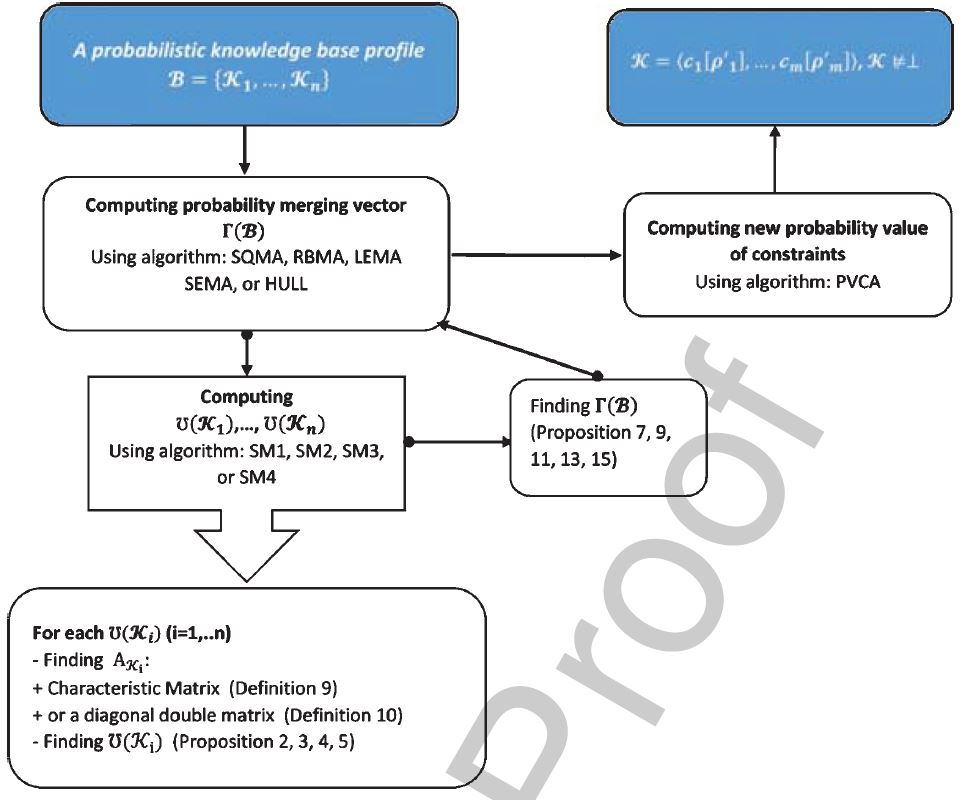
\includegraphics[width=0.5\textwidth]{figure1}
  \end{figure}

  \subsection{Example}

  To illustrate this merging process presented in Fig. 1, the following example will be considered:

  A hospital makes a survey of depression disease. It assigns doctors who are neurologists to this survey.

  These doctors provide the result in which the probability that people has depression disease (denoted by D) are, respectively, 0.7, 0.5, 0.5, 0.8, and 0.6; the probability that people always have sleep problems Fig. 1. The process of merging PKBs.
  (denoted by S) are, respectively, 0.6, 0.5, 0.7, 0.7, and 0.8; the probability that people often feel life’s not worth living (denoted by L) are, respectively, 0.5, 0.5, 0.5, 0.6, and 0.6; the probability that a person has depression disease when that person who has always sleep problems are, respectively, 0.8, 1, 0.6, 0.75, and 0.7; and the probability that a person often feel life’s not worth living, given that he has depression disease are, respectively, 0.8, 1, 0.4, 0.75, and 0.5.

  One of algorithms SM1, SM2, SM3, and SM4 is employed to find a set of probability function values satisfying $\mathcal{K}_i, i = 1, ..., 5$. Then, one of algorithms SQMA, RBMA, LEMA, SEMA, HULL is employed to find a set of probability function values representing newly merged knowledge base. Finally, the PCVA is employed to compute new probability value of constraints in merged knowledge base.

  Table 1 shows these values when the SQMA, LEMA, SEMA are employed while Table 2 shows these values when the RBMA with different values of r and the HULL with different values of $\vec{\lambda}$ are employed. The new PKB which are merged from $\mathcal{K}_1,\mathcal{K}_2,\mathcal{K}_3,\mathcal{K}_4$ is a consistent PKB represented by a probability function satisfying desirable properties. It is evident that the sum of the probability functions of the new PKB equals 1, that is, satisfies Definition 1 about the total of the probability of complete conjunctions over the set of events.

  The detail for explaining the merging process and evaluating algorithms in this paper can be found in an online appendix \footnote{https://vtn82.blogspot.com/2019/04/jifs.html}



  \begin{table*}
    \caption{Original PKBs and merged knowledge bases for algorithms SQMA, LEMA, and SEMA}
    \begin{tabular}{c c c c c c c c c }
      \hline
      $\kappa$ & $\mathcal{K}_1$ & $\mathcal{K}_2$ & $\mathcal{K}_3$ & $\mathcal{K}_4$ & $\mathcal{K}_5$
      & SQMA
      & LEMA
      & SEMA
      \\
      \hline
      (D)   & 0.7 & 0.5 & 0.5 & 0.8  & 0.6 & 0.6403020 & 0.6500584 & 0.8726884 \\
      (S)   & 0.6 & 0.5 & 0.7 & 0.7  & 0.8 & 0.6579282 & 0.7000438 & 0.2585991 \\
      (L)   & 0.5 & 0.5 & 0.5 & 0.6  & 0.6 & 0.5020782 & 0.5500159 & 0.2085848 \\
      (S|D) & 0.8 & 1   & 0.4 & 0.75 & 0.5 & 0.7890107 & 0.7231369 & 0.2041572 \\
      (D|L) & 0.8 & 1   & 0.6 & 0.75 & 0.7 & 0.7423151 & 0.6137144 & 0.6233821 \\
      \hline
    \end{tabular}
  \end{table*}

  \begin{table*}[htb]
    \caption{Merged knowledge bases for algorithms RBMA and HULL}
    \begin{tabular}{l c c c c c c c c}
      \hline
      {$\kappa$} & \multicolumn{3}{c}{RBMA} & \multicolumn{3}{c}{HULL} \\
      & \multicolumn{3}{c}{r} & \multicolumn{3}{c}{$\vec{\lambda}$} \\
      & 1.2        & 1.5        & 2          & (0.2, 0.2, 0.2, 0.2, 0.2) & (0.1, 0.2, 0.3, 0.3, 0.1) & (0.5, 0, 0, 0, 0.5) \\
      \hline
      (D)     & 0.59246940 & 0.60675762 & 0.64030201 & 0.62000000                & 0.62000000                & 0.65000000\\
      (S)     & 0.64011368 & 0.64590239 & 0.65792817 & 0.66000000                & 0.66000000                & 0.70000000\\
      (L)     & 0.51766261 & 0.51297004 & 0.50207822 & 0.54000000                & 0.54000000                & 0.55000000\\
      (S$|$D) & 0.77227016 & 0.77914565 & 0.78901069 & 0.76774194                & 0.75483871                & 0.75384615\\
      (D$|$L) & 0.67921817 & 0.69614187 & 0.74231507 & 0.68518519                & 0.67592593                & 0.63636364          \\
    \end{tabular}
  \end{table*}


  \section{Conclusion}

  In this paper, a new distance-based approach to implement the process of merging PKBs was proposed. The probabilistic MOs based on divergence concepts have been taken under deep consideration and adapted to new probabilistic merging framework by building distance functions between probabilities of constraints. Propositions to calculate the satisfied probabilistic functions of original knowledge bases, probability merging vector, and new probability of constraints in merged PKB were also proposed and proven. Then, postulates about logical relationships between the family of MOs and desirable properties were given. Finally, computational propositions were employed to build merging algorithms. The key differences between the proposed method and existing ones are that input knowledge bases and the merged knowledge base are represented by probabilistic constraints, and our method is considered in a sample space context. However, the input of merging algorithms was PKBs required to be in the same form. Therefore, in the future, new methods will be going on investigating to allow the original knowledge bases to vary in form.


  \section*{Acknowledgment}

  This work has been supported by Vietnam National University, Hanoi (VNU), under Project No. QG.19.23. The authors would like to thank Professor Quang Thuy Ha and Knowledge Technology and Data Science Lab, Faculty of Information Technology, VNU - University of Engineering and Technology for expertise support.

  \bibliography{Output}

\end{document}
